\documentclass[12pt]{article}
\usepackage[a4paper, top=0.8in, left=0.8in, right=0.8in, bottom=0.6in]{geometry}
\usepackage[utf8]{inputenc}
\usepackage{hyperref}
\usepackage{tikz}
\usepackage{float}
\usepackage{multirow}
\usepackage{pifont}
\usepackage{amsmath}
\usepackage{pdflscape}
\usepackage{amssymb}
\usepackage[export]{adjustbox}
\usepackage[backend=biber,style=numeric,sorting=none,sortcites,backref,hyperref]{biblatex}
\addbibresource{references.bib}

\makeatletter
\renewcommand\footnotesize{\scriptsize}
\makeatother

\newcommand{\citerel}{\overset{\mathit{cite}}{\rightarrow}}
\newcommand{\nociterel}{\overset{\mathit{cite}}{\nrightarrow}}

\title{Recommender System for Research Papers \newline\newline \small Group 17}
\author{
  Matthias Bergmann (12219019) \and Maximilian Herczegh (12306066) \and Alexander Scheucher (12113826) \and
    Patrick Ziegler (12303709)
}
\date{\today}

\begin{document}

\maketitle

\begin{abstract}
  With the ever-growing amount of research papers being published, it becomes increasingly difficult for researchers to
  stay updated in their respective fields and discover relevant literature. To address this challenge, we propose the
  development and evaluation of a recommender system specifically designed to suggest relevant research papers based on
  abstract-style textual user queries. In particular, we aim to evaluate the performance of various pre-trained embedding
  models, fine-tuned variations and different retrieval techniques (such as the use of a separate model to re-rank
  approximate k-nearest neighbors) in the context of recommending research papers.\\ Our overarching research question
  is:
  \emph{How well do different combinations of transformer-based
    embedding models and re-ranking models perform for research paper recommendation when evaluated on citation-based
    benchmarks?}
\end{abstract}

\begin{figure}[H]
  \centering
  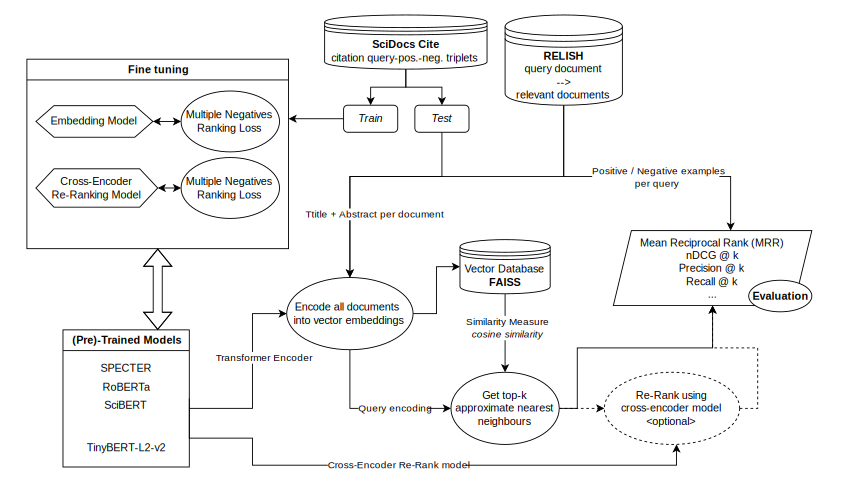
\includegraphics[width=\textwidth]{AIR_schematic_new.pdf}
  \caption{System schematic of the proposed paper recommender and evaluation pipeline.}
  \label{fig:air-schematic}
\end{figure}

\newpage

\section{Introduction}

Using transformer-based embedding models for text representation and information retrieval has become increasingly
popular in recent years. In particular, models such as BERT~\cite{devlin-etal-2019-bert} and its variants have
demonstrated remarkable performance on embedding tasks. Furthermore, the task of recommending research papers on a
given context has gained significant attention due to the growing volume of scientific literature.

In this report, we evaluate how models fine-tuned on citation-based datasets perform in the context of recommending
research papers. We explore various combinations of embedding models and retrieval techniques, including the use of
re-ranking models to enhance the quality of the retrieved results.

\section{Related Work}

Cohan et al.~\cite{cohan-etal-2020-specter} introduced SPECTER, a model specifically designed for generating
document-level embeddings of scientific papers based on the title and abstract. Singh et
al.~\cite{Singh2022SciRepEvalAM}
created SciRepEval, a larger benchmark dataset with multiple tasks for evaluating and comparing scientific paper
representation models to address the reliance on citation-based supervision. This also includes
RELISH~\cite{brown2019large}, an expert annotated dataset for research paper recommendations.

Multiple pre-trained transformer-based models have been proposed for scientific text, such as
SciBERT~\cite{beltagy-etal-2019-scibert}. Furthermore, the use of small cross-encoders, such as
TinyBERT~\cite{jiao-etal-2020-tinybert}, for re-ranking retrieved documents has been shown to improve retrieval
performance in multiple domains~\cite{nogueira2019multi}.

We build upon these works and directly compare these existing fine-tuned models and cross-encoders for the task of
research paper recommendation within a unified framework.

\section{Experiments and Results}

\subsection{Datasets}

We are using the citation-triplets dataset from SciRepEval~\cite{Singh2022SciRepEvalAM} for fine-tuning and evaluating
our models. Each sample in this dataset consists of a
query paper $\mathcal{P}^Q$, a positive paper $\mathcal{P}^+$ and a negative paper $\mathcal{P}^-$. Each paper contains
the title and an abstract. The train set contains around 6.2 million triplets, while the evaluation set contains around
176k triplets. On average, each query paper is part of 10 triplets. The positive paper is a paper
cited by the query paper, thus $\mathcal{P}^Q \citerel \mathcal{P}^+$. The negative papers consist of hard and easy
negatives. Hard negatives are papers that are not cited by the query paper, but are cited by a paper that is cited by
the query paper. Thus, a paper $\mathcal{P}^H$ is a candidate hard negative if there is an intermediate paper
$\mathcal{P}^I$ such that $\mathcal{P}^Q \citerel \mathcal{P}^I \citerel \mathcal{P}^H$ and $\mathcal{P}^Q \nociterel
  \mathcal{P}^H$. Easy negatives are randomly sampled papers that are not cited by the query paper.

To evaluate how a citation based recommender system transfers to real world recommendations we evaluate all our models
on the RELISH dataset~\cite{brown2019large}. This dataset contains
expert annotated relevance judgements for research paper recommendations in the biomedical domain. It contains around
3k queries, each with 60 ranked documents on average. Each query and document contains the title and abstract.
Following the convention of Brown and Yaoqi~\cite{brown2019large}, we consider documents marked \textit{relevant} as
positives and \textit{somewhat-relevant} and \textit{irrelevant} as negatives.

To ensure no data leakage occurs, we use the pre-existing train / evaluation split of the citation-triplets dataset and
removed all papers in its training set that are also present in the RELISH dataset.
\texttt{ir\_measures}\cite{ir-measures-2022}.

\subsection{Models and Methods}

The base models used for embedding generation are SPECTER~\cite{cohan-etal-2020-specter},
SciBERT~\cite{deka2021unsupervised} and a RoBERTa base model~\cite{reimers-2019-sentence-bert} as available on
Huggingface.
The cross-encoder used to re-rank the approximate nearest neighbor results is
TinyBERT-L2-v2~\cite{jiao-etal-2020-tinybert} from
Huggingface. These models are all
implemented using the \texttt{Sentence Transformers} library~\footnote{\url{https://sbert.net/}} and thus easily
interchangeable and fine-tunable.

\subsubsection{Fine-Tuning}

For testing the effect of fine-tuning, we fine-tune the RoBERTa base model on the citation-triplets dataset. We employ
a \texttt{MultipleNegativesRankingLoss}\cite{henderson2017efficient} loss function working directly on the
query-positive-negative triplets. This loss function maximizes the similarity between the query and positive sample,
while minimizing the similarity between the query and all other in-batch samples (negatives). This happens by embedding
each document separately and employing a cross entropy loss on the pairwise cosine similarities. Based on the available
GPU compute, we fine-tune for one full epoch with a batch size of 40, 16-bit precision, learning-rate warmup for 500
steps and weight decay of 0.01, with all
other parameters as default.

The cross-encoder TinyBERT-L2-v2 is fine-tuned using the same parameters and loss function. However, this model
directly outputs the similarity between the query and other documents, as it processes both texts jointly.

\subsubsection{Recommender System}
For each model combination to evaluate, we create a recommender system that first encodes all documents in the
evaluation set using the embedding model. Title and abstract are concatenated with a \texttt{[SEP]} token to form the
representation of a document passed to the model. These embeddings are then stored in a FAISS~\cite{johnson2019billion}
index to allow for efficient
approximate nearest neighbor search. For each query, we first retrieve the top-k nearest documents using the embedding
model. If a re-ranking model is used, these documents are re-ranked using the predicted relevance between the query
and each document. Finally, the top-k documents are returned as
recommendations. By default, we use $k=20$ when evaluating a single embedding model and $k=30$ when using a re-ranking
model to ensure enough documents are available for re-ranking.

\subsection{Evaluation Metrics}
For each dataset, all documents and queries of the evaluation set are embedded using the respective embedding model.
For each query, we retrieve the top-k (optionally re-ranked) documents. This is repeated for every combination of our
four embedding models (SPECTER, SciBERT, RoBERTa, RoBERTa Fine-Tuned) and three re-ranking settings (no re-ranking,
TinyBERT, TinyBERT Fine-Tuned). All obtained query-document rankings are evaluated using standard information retrieval
metrics:
\textit{Success@k}, \textit{Mean Reciprocal Rank (MRR)}, \textit{Normalized Discounted Cumulative Gain (nDCG) @ k},
\textit{Mean Average Precision (MAP)}, \textit{Precision@k} and \textit{Recall@k} using the \texttt{ir\_measures}
library~\cite{zhu2004recall,jarvelin2002cumulated}. These metrics are calculated at multiple cutoff vales
($k\in\{1,5,10\}$) and reported at $k=10$ in Table~\ref{tab:metrics-relish} and Table~\ref{tab:metrics-scirepeval}.
Additionally, we employ query-level bootstrapping with 1000 iterations to obtain
90\% confidence intervals for all metrics.

\section{Conclusion and Results}

Full evaluation results for all model combinations on both datasets with corresponding confidence intervals are shown
in Appendix A (Table~\ref{tab:metrics-relish} and Table~\ref{tab:metrics-scirepeval}). As can be seen in
Figures~\ref{fig:scidocs-ndcg} and~\ref{fig:relish-ndcg}, the use of a re-ranking model consistently improves nDCG@10
scores on both datasets. This supports the hypothesis that re-ranking retrieved documents using a cross-encoder can
enhance the quality of recommendations and is also seen in the comparison of the MRR scores in
Figures~\ref{fig:scidocs-mrr} and~\ref{fig:relish-mrr}.

Furthermore, we managed to replicate the results of Cohan et al.~\cite{cohan-etal-2020-specter} by matching the scores
achieved by SPECTER with our fine-tuned RoBERTa base model on the SciDocs-Cite dataset as well as on the RELISH
dataset.

As expected, the performance of the SciBERT model is lower than that of SPECTER, but still significantly better than
the RoBERTa base model. This indicates that citation based fine-tuning (as is done in SPECTER but not in SciBERT) is
crucial for good performance in the context of research paper recommendation.

When comparing the different re-ranking strategies, we observe that using the pre-trained TinyBERT cross-encoder
consistently improves performance across all embedding models and datasets. Fine-tuning the TinyBERT model on the
citation-triplets dataset results in a decrease in nDCG@10 scores for all embedding models on both datasets. This
indicates that the fine-tuned TinyBERT model does not generalize well to the research paper recommendation task,
possibly due to overfitting or misalignment between the training objective and the evaluation metrics. However, as can
be seen in Figure~\ref{fig:relish-mrr}, the fine-tuned TinyBERT model does improve MRR scores for the RELISH dataset.
This suggests that the fine-tuned re-ranking model focuses more on ranking the top documents correctly, while the
overall ranking quality (as measured by nDCG@10) decreases, which is easier if there are more relevant documents per
query (as is the case in RELISH).

Overall, our experiments demonstrate the effectiveness of transformer-based embedding models and re-ranking techniques
for research paper recommendation. Comparing the results on both datasets, we observe that the performance on the
RELISH dataset is generally higher than on the SciRepEval dataset. While this supports the effectiveness of
citation-based pre-training for research paper recommendation, the disparity is likely influenced by dataset
characteristics, such as domain specificity and the higher number of relevant documents per query in RELISH.

\subsection{Limitations and Future Work}
Although, we carefully cleaned the datasets to minimize data leakage, there is still a chance that some documents from
the RELISH dataset are present in the training set of the citation-triplets dataset or have been used during the
pre-training of the embedding models.

Due to limited computational resources and large dataset size, we could not employ hyperparameter tuning or extensive
experiments on fine-tuning strategies. Thus, the fine-tuning process could be further optimized to improve performance.

Additionally, due to the limited availability of high-quality expert annotated datasets for research paper
recommendation, we could only evaluate on the RELISH dataset which is limited to the biomedical domain. Thus, the
generalization of our results to other scientific domains is limited.

Therefore, we suggest that future work should focus on obtaining larger and more diverse expert annotated datasets
based on real user interactions. Furthermore, exploring more variations of fine-tuned models and different re-ranking
techniques could provide further insights into the optimal configurations for research paper recommendation systems.

\begin{landscape}

\section*{Appendix A: Evaluation Results}

\begin{table}[ht]
  \centering
  \renewcommand{\arraystretch}{1.25}
\begin{tabular}{|l|l|c|c|c|c|c|}
\hline
\textbf{Model} & \textbf{Reranker} & \textbf{MRR} & \textbf{nDCG@10} & \textbf{MAP} & \textbf{Recall@10} & \textbf{Precision@10}\\
\hline
\hline
\multirow{3}{*}{RoBERTa} & None & 51.9 (50.8--52.9) & 34.0 (33.2--34.7) & 13.8 (13.4--14.3) & 17.1 (16.6--17.6) & 30.5 (29.7--31.2)\\
\hline
 & TinyBERT & 62.4 (61.4--63.5) & 44.8 (44.0--45.6) & 20.1 (19.5--20.6) & 22.4 (21.9--23.0) & 39.6 (38.9--40.5)\\
 \hline
 & TinyBERT Fine Tuned & 64.2 (63.1--65.4) & 41.7 (40.9--42.5) & 18.5 (18.0--19.0) & 20.5 (19.9--21.0) & 36.2 (35.5--37.0)\\
 \hline
\hline
\multirow{3}{*}{RoBERTa Fine Tuned} & None & 64.4 (63.4--65.3) & 49.3 (48.5--50.1) & 25.0 (24.5--25.6) & 26.7 (26.0--27.3) & 44.6 (43.8--45.4)\\
\hline
 & TinyBERT & 66.7 (65.7--67.7) & \underline{53.7 (52.9--54.4)} & \underline{30.7 (30.1--31.3)} & \textbf{29.2 (28.5--29.8)} & \underline{49.1 (48.3--49.9)}\\
\hline
 & TinyBERT Fine Tuned & \underline{69.2 (68.1--70.2)} & 48.8 (48.0--49.7) & 27.8 (27.3--28.4) & 25.4 (24.9--26.0) & 43.6 (42.8--44.4)\\
\hline
\hline
\multirow{3}{*}{SciBERT} & None & 61.3 (60.3--62.3) & 44.9 (44.1--45.8) & 21.3 (20.8--21.8) & 23.8 (23.2--24.4) & 40.6 (39.8--41.4)\\
\hline
 & TinyBERT & 65.7 (64.7--66.7) & 51.2 (50.4--52.0) & 27.4 (26.8--28.0) & 27.1 (26.5--27.7) & 46.4 (45.6--47.3)\\
\hline
 & TinyBERT Fine Tuned & 67.5 (66.5--68.6) & 46.7 (45.9--47.6) & 25.0 (24.4--25.5) & 23.7 (23.2--24.3) & 41.6 (40.8--42.4)\\
\hline
\hline
\multirow{3}{*}{SPECTER} & None & 65.9 (64.9--66.9) & 50.9 (50.2--51.7) & 25.7 (25.2--26.2) & 27.1 (26.5--27.7) & 46.1 (45.3--46.9)\\
\hline
 & TinyBERT & 66.7 (65.7--67.7) & \textbf{54.1 (53.3--54.8)} & \textbf{31.0 (30.4--31.5)} & \underline{29.1 (28.5--29.7)} & \textbf{49.7 (48.9--50.5)}\\
\hline
 & TinyBERT Fine Tuned & \textbf{70.3 (69.3--71.4)} & 50.6 (49.9--51.4) & 28.9 (28.3--29.4) & 26.1 (25.6--26.7) & 45.3 (44.5--46.1)\\
\hline
\end{tabular}
\caption{Evaluation results on the RELISH ranked recommendation dataset for all model combinations and selected metrics including the 90\% confidence interval. Best results per metric are \textbf{bolded}, second best are \underline{underlined}.}
\label{tab:metrics-relish}
\end{table}

\begin{table}[ht]
  \centering
  \renewcommand{\arraystretch}{1.25}
\begin{tabular}{|l|l|c|c|c|c|c|}
\hline
\textbf{Model} & \textbf{Reranker} & \textbf{MRR} & \textbf{nDCG@10} & \textbf{MAP} & \textbf{Recall@10} & \textbf{Precision@10}\\
\hline
\hline
\multirow{3}{*}{RoBERTa} & None & 41.7 (41.2--42.2) & 22.0 (21.7--22.3) & 14.7 (14.5--15.0) & 20.6 (20.4--20.9) & 10.9 (10.8--11.1)\\
\hline
 & TinyBERT & 54.6 (54.1--55.1) & 29.5 (29.2--29.8) & 20.8 (20.5--21.1) & 25.5 (25.2--25.8) & 13.7 (13.5--13.8)\\
 \hline
 & TinyBERT Fine Tuned & 52.5 (52.0--53.0) & 29.1 (28.8--29.4) & 20.2 (20.0--20.5) & 26.0 (25.8--26.3) & 14.0 (13.8--14.1)\\
 \hline
 \hline
\multirow{3}{*}{RoBERTa Fine Tuned} & None & 63.6 (63.1--64.1) & 41.6 (41.3--42.0) & 31.9 (31.6--32.2) & 40.9 (40.6--41.3) & 21.9 (21.7--22.1)\\
\hline
 & TinyBERT & \textbf{67.0 (66.5--67.4)} & \textbf{44.1 (43.7--44.4)} & \textbf{34.4 (34.1--34.7)} & \textbf{42.8 (42.5--43.2)} & \textbf{23.0 (22.8--23.2)}\\
 \hline
 & TinyBERT Fine Tuned & 61.8 (61.4--62.3) & \underline{41.8 (41.5--42.1)} & 32.1 (31.8--32.4) & \underline{42.6 (42.3--43.0)} & \underline{22.9 (22.7--23.1)}\\
 \hline
 \hline
\multirow{3}{*}{SciBERT} & None & 56.1 (55.6--56.6) & 33.6 (33.3--33.9) & 24.5 (24.3--24.8) & 32.1 (31.8--32.4) & 17.3 (17.1--17.4)\\
\hline
 & TinyBERT & 63.2 (62.7--63.7) & 39.0 (38.7--39.4) & 29.3 (29.1--29.6) & 36.4 (36.1--36.7) & 19.6 (19.5--19.8)\\
 \hline
 & TinyBERT Fine Tuned & 59.6 (59.2--60.1) & 38.2 (37.8--38.5) & 28.2 (27.9--28.5) & 37.2 (36.9--37.5) & 20.1 (19.9--20.3)\\
 \hline
\hline
\multirow{3}{*}{SPECTER} & None & 60.5 (60.0--61.0) & 38.6 (38.3--38.9) & 29.3 (29.0--29.6) & 37.4 (37.1--37.8) & 20.0 (19.8--20.2)\\
\hline
 & TinyBERT & \underline{64.6 (64.2--65.1)} & 41.6 (41.3--41.9) & \underline{32.1 (31.8--32.4)} & 39.9 (39.6--40.2) & 21.4 (21.2--21.6)\\
 \hline
 & TinyBERT Fine Tuned & 61.9 (61.5--62.4) & 41.1 (40.8--41.4) & 31.3 (31.0--31.6) & 40.9 (40.6--41.2) & 21.9 (21.7--22.1)\\
 \hline
 \end{tabular}
 \caption{Evaluation results on the SciRepEval citation-triplets dataset for all model combinations and selected metrics including the 90\% confidence interval. Best results per metric are \textbf{bolded}, second best are \underline{underlined}.}
 \label{tab:metrics-scirepeval}
\end{table}

\end{landscape}

\section*{Appendix B: Result Figures}
\begin{figure}[ht]
  \centering
  \includegraphics[width=\paperwidth,center]{../figures/scidocs_cite_nDCG@10.png}
  \vspace{-1em}
  \caption{nDCG@10 scores on the SciDocs-Cite dataset.}
  \label{fig:scidocs-ndcg}
\end{figure}

\begin{figure}[ht]
  \centering
  \includegraphics[width=\paperwidth,center]{../figures/relish_nDCG@10.png}
  \vspace{-1em}
  \caption{nDCG@10 scores on the RELISH dataset.}
  \label{fig:relish-ndcg}
\end{figure}

\begin{figure}[ht]
  \centering
  \includegraphics[width=\paperwidth,center]{../figures/scidocs_cite_MRR.png}
  \vspace{-1em}
  \caption{MRR scores on the SciDocs-Cite dataset.}
  \label{fig:scidocs-mrr}
\end{figure}

\begin{figure}[ht]
  \centering
  \includegraphics[width=\paperwidth,center]{../figures/relish_MRR.png}
  \vspace{-1em}
  \caption{MRR scores on the RELISH dataset.}
  \label{fig:relish-mrr}
\end{figure}

\clearpage

\section*{Appendix C: Huggingface Resources}

\begin{table}[ht]
  \centering
  \begin{adjustbox}{max width=\paperwidth - 0.5in,center}
    \renewcommand{\arraystretch}{1.5}
    \begin{tabular}{|l|l|}
      \hline
      \textbf{Resource Name}         & \textbf{Huggingface Link}                                                          \\
      \hline
      \hline
      \multicolumn{2}{|c|}{\textit{Datasets}}                                                                              \\
      \hline
      SciRepEval (Citation Triplets) & \url{https://huggingface.co/datasets/allenai/scirepeval/viewer/cite_prediction_new} \\
      \hline
      RELISH                         & \url{https://huggingface.co/datasets/allenai/scirepeval/viewer/relish}              \\
      \hline
      \hline
      \multicolumn{2}{|c|}{\textit{Models}}                                                                                \\
      \hline
      SPECTER                        & \url{https://huggingface.co/sentence-transformers/allenai-specter}                  \\
      \hline
      SciBERT                        & \url{https://huggingface.co/pritamdeka/S-Scibert-snli-multinli-stsb}                \\
      \hline
      RoBERTa Base                   & \url{https://huggingface.co/sentence-transformers/stsb-roberta-base-v2}             \\
      \hline
      TinyBERT (Cross-Encoder)       & \url{https://huggingface.co/cross-encoder/ms-marco-TinyBERT-L2-v2}                  \\
      \hline
    \end{tabular}
  \end{adjustbox}
  \caption{List of datasets and pre-trained models used in this work with their respective sources.}
  \label{tab:huggingface-resources}
\end{table}

\newpage
\clearpage

\printbibliography[title=References]

\end{document}
